\section{Curved validity in the original coupled Meyer map}\label{sec:curved}
The affine-piece certificate does not apply to an exterior disk projection.
Here we derive a different certificate from the original coupled recurrence,
retaining its curvature and both vector memories. The resulting construction
requires no additional screened solves during path validation.

\subsection{A faithful future-driving quotient and its metric}
Let $D$ be the periodic discrete gradient and $D^*=-\operatorname{div}$.
For a branch with $a=\eta/c>0$, define
\[
 S_a=(I+aD^*D)^{-1},\qquad R_r(t)=t-2\Pi_r(t),
\]
where $\Pi_r$ is the pointwise Euclidean disk projection. The exact stored
Meyer state is $(u,w,t_u,t_w)$. Its next pass depends on the primals only
through $s=u+w$:
\begin{align}
 u^+&=S_a\{s+aD^*R_{r_u}(t_u)\},\nonumber\\
 w^+&=S_b\{f-u^++bD^*R_{r_w}(t_w)\},\nonumber\\
 t_u^+&=Du^++\Pi_{r_u}(t_u),\qquad
 t_w^+=Dw^++\Pi_{r_w}(t_w),\qquad s^+=u^++w^+.
 \label{eq:meyerquotient}
\end{align}
For the retained implementation $a=2$ and $b=10$. Thus
$z=(s,t_u,t_w)$ is an exact state for all future passes. Both vector fields,
including their transverse components, remain present. The current primal
difference $u-w$ is not recoverable from this quotient; the next actual pass
recovers both next primals exactly. The emitted texture $f-u-w=f-s$ is
already recoverable at the current state. This is a precise quotient of
redundant state, not deletion of a driving memory variable.

\begin{theorem}[Metric of the coupled recurrence]\label{thm:meyermetric}
The quotient map $F$ in \eqref{eq:meyerquotient} is nonexpansive in
\begin{equation}
 \norm{z}_M^2=\norm{s}_2^2+a\norm{t_u}_2^2+b\norm{t_w}_2^2.
 \label{eq:meyermetric}
\end{equation}
In fact, for any two states $z,\widetilde z$,
\begin{equation}
 \norm{Fz-F\widetilde z}_M^2+
 \tfrac12\norm{(I-F)z-(I-F)\widetilde z}_M^2
 \leq\norm{z-\widetilde z}_M^2. \label{eq:meyeraveraged}
\end{equation}
Equivalently, this map is $2/3$-averaged. The statement does not require
the input states to lie on an ordinary proximal trajectory.
\end{theorem}
\begin{proof}
On pairs $(y,t)$ with norm $\norm{y}^2+a\norm{t}^2$, let $P_{\mathcal G_a}$
be the orthogonal projection onto the graph $\mathcal G_a=\{(x,Dx)\}$.
Its first component on $(y,R_r(t))$ is
$v=S_a(y+aD^*R_r(t))$. Therefore the branch map
\[
 A_a(y,t)=(v,Dv+\Pi_r(t))
 =\tfrac12\{I+(2P_{\mathcal G_a}-I)\operatorname{diag}(I,R_r)\}(y,t)
\]
is firmly nonexpansive: graph reflection is an isometry, and $R_r$ is
nonexpansive by firm nonexpansivity of disk projection.

Write differences between two inputs and outputs with a $\Delta$; in the
following inequalities, $u,w$ denote the updated primals.
The first branch gives
\[
 \norm{\Delta u}^2+a\norm{\Delta t_u^+}^2
 \leq\norm{\Delta s}^2+a\norm{\Delta t_u}^2
 -\norm{\Delta(s-u)}^2-a\norm{\Delta(t_u-t_u^+)}^2.
\]
Firm nonexpansivity of the second branch, whose input difference is
$(-\Delta u,\Delta t_w)$, gives
\[
 \norm{\Delta w}^2+b\norm{\Delta t_w^+}^2
 \leq-\ip{\Delta w}{\Delta u}+b\ip{\Delta t_w^+}{\Delta t_w}.
\]
Rearranging twice this inequality shows
\[
 \norm{\Delta(u+w)}^2+b\norm{\Delta t_w^+}^2
 \leq\norm{\Delta u}^2+b\norm{\Delta t_w}^2
 -\norm{\Delta w}^2-b\norm{\Delta(t_w-t_w^+)}^2.
\]
Combining the two bounds proves nonexpansivity. Finally,
\[
 \norm{\Delta(s-u)}^2+\norm{\Delta w}^2
 \geq\tfrac12\norm{\Delta(s-u-w)}^2
\]
yields \eqref{eq:meyeraveraged} with the two vector-memory terms.
\end{proof}

Whitening this metric gives ordinary Euclidean Arnoldi on the five scalar
fields $(s,\sqrt a\,t_u,\sqrt b\,t_w)$. Fixed finite polynomials in this
metric differ from the earlier six-field Euclidean implementation; the
experiments retain both, separating the representation change from discovery.

\subsection{Exact algebraic description of disk curvature}
For an anchor vector $t=\rho n$, choose an orthonormal frame $(n,e)$ and
write a reduced displacement as $h=h_n n+h_t e$. Both $h_n$ and $h_t$ are
linear forms in the Krylov coordinates $c$. The new squared radius is
\begin{equation}
 \ell(c)^2=(\rho+h_n(c))^2+h_t(c)^2. \label{eq:diskradicand}
\end{equation}
It is a quadratic polynomial. The disk event is the inequality
$\ell(c)^2\leq r^2$; normalization introduces its positive square root.
These relations can be acquired once from the anchor and basis.

Let $q=\Pi_r(t+h)-\Pi_r(t)-P_t h$, where $P_t$ is the selected linear
projection action used by Arnoldi. For an interior anchor, including the
implementation's identity selection at $\rho=r$,
\begin{equation}
 \norm{q}^2=(\ell-r)_+^2. \label{eq:diskinside}
\end{equation}
For an exterior anchor $\rho>r$, put $\sigma=\min(1,r/\ell)$, with
$\sigma=1$ at $\ell=0$. Then
\begin{equation}
 q_n=\sigma(\rho+h_n)-r,\qquad
 q_t=(\sigma-r/\rho)h_t. \label{eq:diskoutside}
\end{equation}
These are exact identities on both sides of a crossing. In particular,
pure radial motion on the same exterior ray has zero remainder while
turning generally does not. A constant inside/outside mask alone fails to
capture this distinction. At nonsmooth boundary anchors, the argument uses
the specified linear action and exact remainder, not a nonexistent classical
Jacobian.

Only two linear forms per disk site are needed to evaluate
\eqref{eq:diskradicand}--\eqref{eq:diskoutside}. The proposed representation
is therefore a finite collection of polynomial radicands, branch inequalities,
and radial normalization relations. It does not claim global finite closure
of the nonlinear iteration in a polynomial observable dictionary.

\subsection{The nonlinear remainder has a fixed linear response}
Let $q_u,q_w$ be the exact projection remainders at a candidate displacement.
The corresponding remainder of the complete map has primal components
\begin{align}
 d_u&=-2aS_aD^*q_u,\nonumber\\
 d_w&=-S_b d_u-2bS_bD^*q_w,
 \label{eq:curveresponse}
\end{align}
and quotient components
$(d_u+d_w,Dd_u+q_u,Dd_w+q_w)$. Thus all nonlinear curvature is confined
to the two pointwise projection remainders; the rest is a fixed linear
response. We do not evaluate the screened solves in \eqref{eq:curveresponse}
for each predicted point. Instead, their operator norm supplies a bound.

For a discrete Laplacian eigenvalue $\lambda$, longitudinal components of
this response, after whitening, have Gram matrix
\[
 G(\lambda)=\begin{pmatrix}1-d(\lambda)&g(\lambda)\\g(\lambda)&1\end{pmatrix},
\quad
 d(\lambda)=\frac{4a\lambda}{(1+a\lambda)^2(1+b\lambda)},\quad
 g(\lambda)=\frac{2\sqrt{ab}\lambda}{(1+a\lambda)(1+b\lambda)}.
\]
Transverse components have gain one. Consequently, with
\begin{equation}
 \gamma^2=\max_{\lambda\in\operatorname{spec}(D^*D)}
 \left[1-\frac{d(\lambda)}2+
 \sqrt{\frac{d(\lambda)^2}4+g(\lambda)^2}\right], \label{eq:curvegain}
\end{equation}
we have
\begin{equation}
 \norm{N(v)}_M\leq
 \gamma\sqrt{a\norm{q_u(v)}_2^2+b\norm{q_w(v)}_2^2}.
 \label{eq:curvebound}
\end{equation}
This is a grid- and parameter-dependent calculation, independent of the
source image. For the retained $64\times64$ grid, $\gamma=1.14819$.
The Gram formula follows by Fourier diagonalization of
\eqref{eq:curveresponse}; the two transverse components pass unchanged.
Independent tests compare the full nonlinear remainder against the linear
response and its norm bound.

\begin{theorem}[Curved Meyer path certificate]\label{thm:curvedpath}
For an $M$-orthonormal Arnoldi basis, let $E=JQ-QH$,
$c_0=0$, $c_{j+1}=\beta e_1+Hc_j$, and
$\widehat z_j=z+Qc_j$. Define
\[
 \varepsilon_j=\norm{Ec_j}_M+
 \gamma\sqrt{a\norm{q_u(Qc_j)}^2+b\norm{q_w(Qc_j)}^2}.
\]
Then, for every finite horizon,
\begin{equation}
 \norm{F^m(z)-\widehat z_m}_M
 \leq\sum_{j=0}^{m-1}\varepsilon_j. \label{eq:curvedpath}
\end{equation}
The same bound controls the emitted texture error. It also remains valid
after a common ordinary settling step. No fixed-mask assumption is required.
\end{theorem}
\begin{proof}
The exact defect is $N(Qc_j)+Ec_j$. Apply \eqref{eq:curvebound} and the
triangle inequality, then propagate errors by Theorem~\ref{thm:meyermetric}.
The initial error is zero, so summation gives \eqref{eq:curvedpath}.
Texture is $f-s$ and its error norm is bounded by the full quotient norm.
A common settling step cannot increase the quotient error.
\end{proof}

All projection remainders along the predicted path are evaluated; this is
not sparse sampling of a few convenient points. The reduction is algebraic:
small-coordinate evaluation and pointwise radial operations replace repeated
screened solves. Compression norms use the small matrix $E^TME$.
The certificate is proved in exact arithmetic and tested in floating point;
we do not claim outward-rounded numerical certification.

\subsection{Coverage, local amortization, and complete solves}

The retained coverage battery uses camera, Barbara, a histogram-preserving camera permutation, a straight carrier, and crossing carriers with an edge, all at $64\times64$. Ordinary anchors are taken after $4,32,128,512$ passes, with depths $2,4,8$ and horizons $8,16,32,64$. All 240 measured quotient errors satisfy \eqref{eq:curvedpath} within numerical tolerance. The texture errors after settling are independently checked as well. The certificate is an analytic bound; these finite tests verify its implementation rather than establish the theorem.

For example, at camera prefix $512$, depth two and horizon sixteen, the bound is $0.0954$ times predicted displacement and the actual error is $0.019$ times actual displacement. At camera prefix four the same horizon has a much larger curvature budget. Increasing depth can reduce compression without removing that changing geometry.

The live discovery policy acquires depths $2,4,8$ incrementally and checks the reduced path in chunks of eight up to horizon $64$. It stops a depth after the first chunk whose accumulated bound exceeds $0.1$ times predicted displacement, then selects a checked horizon whose nominal operator savings exceed $1.5\times$ acquisition and settling work. This early stopping rule need not find the longest admissible horizon. It does not consult a future trajectory or gap oracle.

The policy accepts seven of the twenty anchors. With five timing repeats, the late camera block discovers depth two/horizon sixteen and is $1.39\times$ faster than ordinary replay. The straight carrier at prefixes $128$ and $512$ discovers depth two/horizon sixty-four and gives $3.47\times$ and $3.48\times$ speedups. Three of the seven accepted blocks are slower despite passing the nominal work screen. Timings include chart acquisition, radial checks, reconstruction, and one settling pass for both methods.

\begin{figure}[htbp]\centering

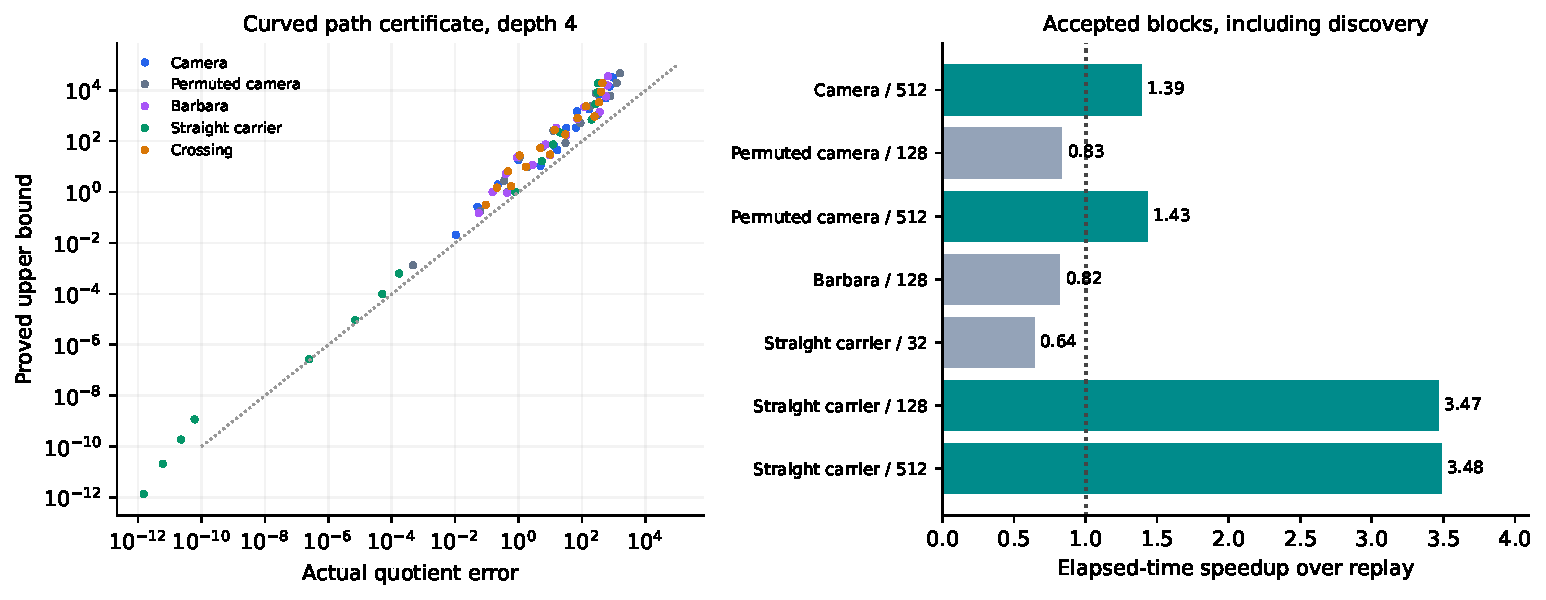
\includegraphics[width=\textwidth]{figures/curved_validity.pdf}

\caption{Left: independently replayed errors and the curved certificate for depth four, across all anchors and horizons. The dotted diagonal is equality; plotting floors are $10^{-12}$. Right: all seven accepted live-discovery blocks, labeled by source and ordinary anchor prefix. Thirteen rejected anchors remain in the raw records.}

\end{figure}

For complete solves, all methods use the same original recurrence and the same recovered primal--dual gap. The target is $10^{-4}$ times the initial gap, checked every thirty-two work units. The fixed methods use depth four, horizon sixteen, and one settling pass; they differ only in six-field Euclidean versus whitened quotient coordinates. The discovered method takes thirty-two ordinary steps after an unprofitable acquisition. Its fallback also charges an additional pass to recover the full primal output. The work ceiling is 4096; all methods reach the target on every source.

\begin{table}[htbp]\centering\small

\begin{tabular}{l rrrr}\toprule

Source & Ordinary & Fixed, six fields & Fixed, quotient & Discovered\\\midrule

Camera & 229.9 & 407.7 & 419.9 & 386.3\\

Permuted camera & 32.8 & 78.9 & 76.0 & 63.4\\

Barbara & 98.2 & 154.1 & 174.3 & 187.2\\

Straight carrier & 24.6 & 36.7 & 46.4 & 53.6\\

Crossing & 174.8 & 172.2 & 263.2 & 279.7\\

\bottomrule\end{tabular}

\caption{Complete Python solve milliseconds on the M4 Mini, one BLAS thread, median of three shuffled timed runs after warm-up. Setup is excluded; gap checks, discovery, rejected candidates, and all update work are included. These are not native-kernel timings.}

\label{tab:curvedsolve}\end{table}

The conservative discovered policy loses to ordinary iteration on all five complete solves, despite profitable certified blocks in some later regimes. This is a retained negative result. A valid curved description is now available for the original map; the current acquisition policy and sufficient path-error bound are not yet an economical general accelerator. As in the earlier Meyer probe, successful acceleration need not closely reproduce the entire ordinary trajectory. The strict certificate is a controlled research instrument, not a replacement imposed on the established native operator.

The continuation suite passes 41 tests, including the exact future-driving quotient, the stronger averaged-map inequality, curvature formulas across boundary events, sharp attainment of the Fourier response gain, and independently replayed path bounds.

